\section{Moduli Spaces of Curves} \label{baseS}

Fix $g \in \N$ and $h \in \Z_+$. In the remaining sections we examine the moduli space of holomorphic curves with main component $(u_0,\Sigma_0)$ and topological type $(g,h)$. 
In each case the domain is modeled on a tree with root $\Sigma_0$ and (possibly nodal) constant branches. These curves are indexed by the distribution of genus and boundary components across ghost branches.

\begin{figure}[ht]
\centering
\begin{tikzpicture}

% sigma0
\coordinate (sigma0) at (0,0);
\def\rzero{2}
\disk[](sigma0)(\rzero)(1.5*\rzero);
\begin{scope}[shift=(sigma0)]
	\node [below] at (0,-0.5) {$\Sigma_0$};
\end{scope}

% sigma1
\coordinate (node1) at ($(sigma0)+(-1.49,2)$);
\def\rone{2}
\torus[](node1)(50)(\rone)
\begin{scope}[shift=(node1), rotate around={50:(node1)}]
    \node [above left] at ($(node1)+(0,2*\rone)$) {$\Sigma_1$};
\end{scope}

% sigma2
\coordinate (node2) at ($(sigma0)+(1,2.6)$);
\def\rtwo{1}

\begin{scope}[shift=(node2), rotate around={-30:(node2)}]
    \coordinate (node2a) at (-0.707*\rtwo,1.707*\rtwo);
    \coordinate (node2b) at (0.707*\rtwo,1.707*\rtwo);
    \sphere[](0,\rtwo)(\rtwo)(\rtwo);
    \node at (0,0) {$\bullet$};
    \torus[](node2a)(40)(1);
    \closedGhost[](node2b)(-30)(1.2)(1.6)(2);
    \node [left] at (0,3) {$\Sigma_2$};
\end{scope}

% sigma3
\coordinate (node3) at ($(sigma0)+(\rzero,0)$);
\openGhost[](node3)(1.5)(2)(2)();
\begin{scope}[shift=(node3)]
	\addGenus[](1.5,1.1)(0)(0.5)
	\node at (1.5,-0.5) {$\Sigma_3$};
\end{scope}

\end{tikzpicture}
\caption{A curve with three ghost branches, modeled on $(1,3,(1,2))$.}
\end{figure}

\begin{definition} \label{partNum}
Fix $g \in \mathbb{N}$ and $h \in \Z_+$. A \emph{partition} of $(g,h)$ is an ordered choice of $\{g_1,\ldots,g_r\}$ and $\{(g_{r+1},h_{r+1}),\ldots,(g_{r+q},h_{r+q})\}$ for some $r,q \geq 0$ so that
\begin{align*}
g & = 0+g_1+\ldots+g_k
\\
h & = 1+(h_{r+1}-1)+\ldots+(h_k-1).
\end{align*}
We require
\begin{enumerate}[(i)]
\item $g_i \geq 1$ for $i \leq r$ and
\item $g_i \geq 0$, $h_i \geq 1$, and $2g_i+h_i-1 \geq 1$ for $i>r$.
\end{enumerate}
\end{definition}

\begin{remark}
Two partitions are equivalent if they are the same up to re-ordering. However, we will ignore this equivalence until Section~\ref{calcS}. We will order partitions so that all the closed ghosts appear before the open ghosts for the sake of notational clarity.
\end{remark}

\begin{definition} \label{partition}
Fix a partition $\lambda=(g_1,\ldots,g_r,(g_{r+1},h_{r+1}),\ldots,(g_{r+q},h_{r+q}))$ of some topological type $(g,h)$. A \emph{domain modeled on $\lambda$} is a nodal domain $\Sigma \in \Mbar_{(g,h),0,\vec{0}}$ so that
\begin{enumerate}[(i)]
\item $\Sigma_0$ is disk with marked points $\{z_1,\ldots,z_{r+q}\}$ so that $z_i \in \partial\Sigma_0$ if and only if $i>r$,
\item for $1 \leq i \leq r$, $\Sigma_i \in \Mbar_{g_i,1}$ is a closed curve with marked point $y_i$,
\item for $r+1 \leq i \leq r+q$, $\Sigma_i \in \Mbar_{(g_i,h_i),0,(1,0,\ldots,0)}$ is an open curve with marked point $y_i \in \partial\Sigma_i$, and
\item $\Sigma_i$ is attached to $\Sigma_0$ by identifying marked points:
\[
\Sigma=\left.\left( \bigsqcup\limits_{i=0}^{r+q} \Sigma_i \right) \middle/ (z_i \sim y_i) \right.
\]
\end{enumerate}
We refer to $\Sigma_0$ as the \emph{main component}; the remaining (possibly nodal) curves $\Sigma_1,\ldots,\Sigma_{r+q}$ are \emph{branches}.

A \emph{holomorphic curve modeled on $\lambda$} is a holomorphic map $u:(\Sigma,\partial\Sigma)\arr(M,L)$ so that
\begin{enumerate}[(i)]
\item $\Sigma$ is a domain modeled on $\lambda$,
\item $u_0=u|_{\Sigma_0}$ satisfies Hypothesis~\ref{hypMain}, and
\item the branches $u_i=u|_{\Sigma_i}$ are constant for $i \geq 1$.
\end{enumerate}
\end{definition}

\begin{remark}
If $\Sigma$ is modeled on a partition $\lambda=(g_1,\ldots,g_r,(g_{r+1},h_{r+1}),\ldots,(g_{r+q},h_{r+q}))$ of $(g,h)$, then a smoothing of $\Sigma$ has genus $g$ with $h$ boundary components. The conditions we impose on $g_i$ for $i \leq r$ and on $2g_i+h_i-1$ when $i>r$ exclude unstable ghost branches.
\end{remark}

\begin{definition}
Let $\Lambda$ be the set of all partitions of $(g,h)$. For each $\lambda \in \Lambda$, the \emph{$\lambda$-cell} $\Nbar_\lambda$ is the moduli space of holomorphic curves modeled on $\lambda$. 

The moduli space of curves of type $(g,h)$ is
\[
\Nbar = \bigcup\limits_\Lambda \Nbar_\lambda.
\]
\end{definition}

Each cell of $\Nbar$ is moduli space of curves in the typical sense: it has a fixed dimension, with one top stratum and various lower-dimensional strata corresponding to degenerations of the domain. However, these cells may have $1$-dimensional boundary, and different cells may have different dimensions.

The advantage of decomposing $\Nbar$ in this manner is that individual cells are straightforward. If $\lambda=(g_1,\ldots,g_r,(g_{r+1},h_{r+1}),\ldots,(g_{r+q},h_{r+q}))$, then
\[
\Nbar_\lambda = \prod\limits_{i=1}^{r} (\Sigma_0 \times \Mbar_{g_i,1}) \times \prod\limits_{i=r+1}^{r+q} (\partial\Sigma_0\times\Mbar_{(g_i,h_i),0,(1,0,\ldots,0)}).
\]
Therefore
\[
\dim_\R(\Nbar_\lambda) = \sumto{i=1}{r} (2+2(3g_i-2)) + \sumto{i=r+1}{r+q} (1+3(2g_i+h_i-1)-2) = 3\tilde{g}-(2r+q),
\]
where $\tilde{g}=2g+h-1$ is the genus of the complex double of a curve modeled on $\lambda$.

Cells corresponding to different partitions intersect when the following phenomena occur:
\begin{enumerate}[(i)]
\item ghost branches collide, or
\item an interior ghost branch approaches $\partial\Sigma_0$.
\end{enumerate}
Note that the second type of collision corresponds to a collision of conjugate ghosts in the complex double of a curve. Thus it is possible to understand all of these collisions using standard techniques for closed curves.

Our next goal is to characterize these cell intersections more explicitly. Figures~\ref{collClosedPic}, \ref{collOpenPic}, and \ref{collBdryPic} depict the complex doubles of the three basic intersection types.

If a curve in $\Nbar_\lambda$ has two ghosts attached at $z_i$ and $z_{i'}$, then $\Nbar_\lambda$ intersects another cell when $z_i=z_{i'}$. The collision produces an extra bubble (a sphere in the closed case and a disk in the open case); the resulting ghost branch is a degeneration of a single ghost component attached at $z_i=z_{i'}$ .

If a curve in $\Nbar_\lambda$ has a closed ghost attached at $z_i$, then $\Nbar_\lambda$ intersects another cell when $z_i$ approaches $\partial\Sigma_0$. The collision produces an extra disk bubble; the resulting ghost branch is a degeneration of an open ghost attached at $z_i$.

\begin{enumerate}[(I)]
\item If two closed ghosts $[\Sigma_i,y_i] \in \Mbar_{g_i,1}$ and $[\Sigma_{i'},y_{i'}] \in \Mbar_{g_{i'},1}$ collide, we see a sphere bubble attached to $\Sigma_0$, $\Sigma_i$, and $\Sigma_{i'}$. This is a degeneration of a closed ghost with genus $g_i+g_{i'}$. \label{collisionClosed}
\item If two open ghosts $[\Sigma_i,y_i] \in \Mbar_{(g_i,h_i),0,(1,0,\ldots,0)}$ and $[\Sigma_{i'},y_{i'}] \in \Mbar_{(g_{i'},h_{i'}),0,(1,0,\ldots,0)}$ collide, we see a disk bubble attached to $\partial\Sigma_0$, $\partial\Sigma_i$, and $\partial\Sigma_{i'}$. This is a degeneration of an open ghost of type $(g_i+g_{i'},h_i+h_{i'}-1)$. \label{collisionOpen}
\item If a closed ghost $[\Sigma_i,y_i] \in \Mbar_{g_i,1}$ approaches $\partial\Sigma_0$, we see a disk bubble attached to $\partial\Sigma_0$ and $\Sigma_i$. This is a degeneration of an open ghost of type $(g_i,1)$. \label{collisionBoundary}
\end{enumerate}

\begin{figure}[ht]
\centering
\begin{tikzpicture}[scale=0.5]

\def\r{1.5} % radius
\def\w{5} % distance between curves

%%%%%%%%%%%%%%%%%%%%%%%% collision

\coordinate (coll) at (0,0);

\sphere[](coll)(\r)(\r);

% ghosts
\coordinate (nodeC) at ($(coll)+(0,\r)$);
\node at (nodeC) {$\bullet$};

\begin{scope}[shift=(nodeC), rotate around={30:(nodeC)}]
	\draw (0,0) to [out=60,in=0] (0,3) to [out=180,in=150] (0,0);
    \addGenus[](0,2)(90)(0.5);
\end{scope}
\begin{scope}[shift=(nodeC), rotate around={-30:(nodeC)}]
    \draw (0,0) to [out=120,in=180] (0,3) to [out=0,in=30] (0,0);
    \addGenus[](0,1.2)(0)(0.3);
    \addGenus[](0,2.1)(0)(0.3);
\end{scope}

% conjugate ghosts
\coordinate (negNodeC) at ($(coll)+(0,-\r)$);
\node at (negNodeC) {$\bullet$};

\begin{scope}[shift=(negNodeC), yscale=-1, rotate around={30:(negNodeC)}]
	\draw (0,0) to [out=60,in=0] (0,3) to [out=180,in=150] (0,0);
    \addGenus[](0,2)(90)(0.5);
\end{scope}
\begin{scope}[shift=(negNodeC), yscale=-1, rotate around={-30:(negNodeC)}]
    \draw (0,0) to [out=120,in=180] (0,3) to [out=0,in=30] (0,0);
    \addGenus[](0,1.2)(0)(0.3);
    \addGenus[](0,2.1)(0)(0.3);
\end{scope}

%%%%%%%%%%%%%%%%%%%%%%%% bubble

\coordinate (bubble) at (2*\w,0);

\sphere[](bubble)(\r)(\r);

% ghosts
\coordinate (nodeB) at ($(bubble)+(0,\r)$);
\coordinate (nodeB1) at ($(nodeB)+(-0.3*\r,0.9*\r)$);
\coordinate (nodeB2) at ($(nodeB)+(0.3*\r,0.9*\r)$);

\sphere[]($(nodeB)+(0,0.5*\r)$)(0.5*\r)(0.5*\r);
\node at (nodeB) {$\bullet$};

\torus[](nodeB1)(30)(1.5);

\closedGhost[](nodeB2)(-30)(0.9)(1.5)(2);

% conjugate ghosts
\coordinate (negNodeB) at ($(bubble)+(0,-\r)$);
\coordinate (negNodeB1) at ($(negNodeB)+(-0.3*\r,-0.9*\r)$);
\coordinate (negNodeB2) at ($(negNodeB)+(0.3*\r,-0.9*\r)$);

\sphere[]($(negNodeB)+(0,-0.5*\r)$)(0.5*\r)(0.5*\r);
\node at (negNodeB) {$\bullet$};

\begin{scope}[yscale=-1]
    \torus[](negNodeB1)(30)(1.5);

    \closedGhost[](negNodeB2)(-30)(0.9)(1.5)(2);
\end{scope}

%%%%%%%%%%%%%%%%%%%%%%%% smoothing

\coordinate (smooth) at (4*\w,0);

\sphere[](smooth)(\r)(\r);

% ghost
\coordinate (nodeS) at ($(smooth)+(0,\r)$);
\node at (nodeS) {$\bullet$};

\begin{scope}[shift={(nodeS)}]
\draw (0,0) to [out=0,in=-140] (1,1.6) to [out=40,in=-90] (2.1,2.8) to [out=90,in=0] (1.5,3.6) to [out=180,in=90] (0.7,2.8) to [out=-90,in=0] (0,1.5) to [out=180,in=-90] (-0.7,2.8) to [out=90,in=0] (-1.5,3.6) to [out=180,in=90] (-2.1,2.8) to [out=-90,in=140] (-1,1.6) to [out=-40,in=180] (0,0);
\addGenus[](-1.4,2.8)(120)(0.4);
\addGenus[](1.2,2.34)(-30)(0.3);
\addGenus[](1.5,3.12)(-30)(0.3);
\end{scope}

% conjugate ghost
\coordinate (negNodeS) at ($(smooth)+(0,-\r)$);
\node at (negNodeS) {$\bullet$};

\begin{scope}[shift={(negNodeS)}, yscale=-1]
\draw (0,0) to [out=0,in=-140] (1,1.6) to [out=40,in=-90] (2.1,2.8) to [out=90,in=0] (1.5,3.6) to [out=180,in=90] (0.7,2.8) to [out=-90,in=0] (0,1.5) to [out=180,in=-90] (-0.7,2.8) to [out=90,in=0] (-1.5,3.6) to [out=180,in=90] (-2.1,2.8) to [out=-90,in=140] (-1,1.6) to [out=-40,in=180] (0,0);
\addGenus[](-1.4,2.8)(120)(0.4);
\addGenus[](1.2,2.34)(-30)(0.3);
\addGenus[](1.5,3.12)(-30)(0.3);
\end{scope}

%%%%%%%%%%%%%%%%%%%%%%%% arrows

\def\h{1}
\coordinate (arr1) at ($0.5*(coll)+0.5*(bubble)+(0,\h)$);
\coordinate (arr2) at ($0.5*(bubble)+0.5*(smooth)+(0,\h)$);
\draw [->, bend left] ($(arr1)+(-1,0)$) to ($(arr1)+(1,0)$);
\draw [->, bend right] ($(arr2)+(1,0)$) to ($(arr2)+(-1,0)$);
\node [above=5pt] at (arr1) {\footnotesize reparametrization};
\node [above=5pt] at (arr2) {\footnotesize degeneration};

\end{tikzpicture}
\caption{(I) The collision of genus $1$ and $2$ ghosts as a degeneration of a genus $3$ ghost.}
\label{collClosedPic}
\end{figure}

\begin{figure}[ht]
\centering
\begin{tikzpicture}[scale=0.7]

\def\r{1.5}
\def\w{4} % distance between curves

%%%%%%%%%%%%%%%%%%%%%%%% collision

\coordinate (coll) at (0,0);

\coordinate (nodeC) at ($(coll)+(0,-0.175*\r)$);

\draw (coll) circle (\r);

\begin{scope} % erase main component blocked by left ghost
	\clip ($(nodeC)+(-1.4,0)$) ellipse (1.4 and 0.8);
	\draw [white, fill=white] (coll) circle (\r+1);
	\draw [dashed] (coll) circle (\r);
\end{scope}

\begin{scope} % fill main component in hole of left ghost
	\clip ($(nodeC)+(-1.4,0)$) ellipse (0.5 and 0.3);
	\draw [bend right = 15] ($(coll)+(-\r,0)$) to ($(coll)+(\r,0)$);
	\draw (coll) circle (\r);
\end{scope}

\begin{scope} % erase main component blocked by right ghost
	\clip ($(nodeC)+(1.4,0)$) ellipse (1.4 and 0.8);
	\draw [white, fill=white] (coll) circle (\r+1);
	\draw [dashed] (coll) circle (\r);
\end{scope}

% main component details
\draw [dashed, bend right = 15] ($(coll)+(-\r,0)$) to ($(coll)+(\r,0)$);
\node at (nodeC) {$\bullet$};

\begin{scope}[shift={(nodeC)}]
    % left ghost
	\draw (-1.4,0) ellipse (1.4 and 0.8);
	\draw (-1.4,0) ellipse (0.5 and 0.3);
	\draw [bend right = 15] (-2.8,0) to (-1.9,0);
	\draw [bend right = 15] (-0.9,0) to (0,0);
    
    % right ghost
	\draw (1.4,0) ellipse (1.4 and 0.8);
	\draw [bend right = 15] (0,0) to (2.8,0);
	\addGenus[](0.9,0.5)(20)(0.3);
	\addGenus[](2.1,0.45)(-10)(0.3);
	\addGenus[yscale=-1](0.9,-0.5)(20)(0.3);
	\addGenus[yscale=-1](2.1,-0.45)(-10)(0.3);
\end{scope}

%%%%%%%%%%%%%%%%%%%%%%%% bubble

\coordinate (bubble) at (2*\w,0);
\coordinate (nodeB) at ($(bubble)+(0,-0.175*\r)$);
\coordinate (sphere) at ($(nodeB)+(0,-0.04*\r)$);
\coordinate (nodeB1) at ($(sphere)+(-0.5*\r,0)$);
\coordinate (nodeB2) at ($(sphere)+(0.5*\r,0)$);

\draw (bubble) circle (\r);

\begin{scope} % erase main component blocked by left ghost
	\clip ($(nodeB1)+(-1.4,0)$) ellipse (1.4 and 0.8);
	\draw [white, fill=white] (bubble) circle (\r+1);
	\draw [dashed] (bubble) circle (\r);
\end{scope}

\begin{scope} % erase main component blocked by right ghost
	\clip ($(nodeB2)+(1.4,0)$) ellipse (1.4 and 0.8);
	\draw [white, fill=white] (bubble) circle (\r+1);
	\draw [dashed] (bubble) circle (\r);
\end{scope}

% main component details
\draw [dashed, bend right = 15] ($(bubble)+(-\r,0)$) to ($(bubble)+(\r,0)$);

\node at (nodeB) {$\bullet$};
\node at (nodeB1) {$\bullet$};
\node at (nodeB2) {$\bullet$};

\begin{scope}[shift=(sphere)] % center ghost
	\draw (0,0) circle (0.5*\r);
	\draw [bend right = 15] (-0.5*\r,0) to (0.5*\r,0);
	\draw [dashed, bend left = 10] (-0.5*\r,0) to (0.5*\r,0);
\end{scope}

\begin{scope}[shift={(nodeB1)}] % left ghost
	\draw (-1.4,0) ellipse (1.4 and 0.8);
	\draw (-1.4,0) ellipse (0.5 and 0.3);
	\draw [bend right = 15] (-2.8,0) to (-1.9,0);
	\draw [bend right = 15] (-0.9,0) to (0,0);
\end{scope}

\begin{scope}[shift={(nodeB2)}] % right ghost
	\draw (1.4,0) ellipse (1.4 and 0.8);
	\draw [bend right = 15] (0,0) to (2.8,0);
	\addGenus[](0.9,.45)(20)(0.3);
	\addGenus[yscale=-1](0.9,-0.45)(20)(0.3);
	\addGenus[](2.1,0.45)(-10)(0.3);
	\addGenus[yscale=-1](2.1,-0.45)(-10)(0.3);
\end{scope}

%%%%%%%%%%%%%%%%%%%%%%%% smoothing

\coordinate (smooth) at (4*\w,0);

\coordinate (nodeS) at ($(smooth)+(0,-0.175*\r)$);
\coordinate (sphereS) at ($(nodeS)+(0,-0.04*\r)$);

\draw (smooth) circle (\r);

\begin{scope}[shift={(sphereS)}]
    % use preaction to fix conflict between extra options (white) and clip
	\path[preaction={draw,fill=white}][clip] (0,0.5*\r) to [out=180, in=0] (-0.5*\r,0.4) to [out=180, in=0] (-0.5*\r-1.4,0.8) to [out=180, in=90] (-0.5*\r-2.8,0) to [out=-90, in=180] (-0.5*\r-1.4,-0.8) to [out=0, in=180] (-0.5*\r,-0.4) to [out=0, in=180] (0,-0.5*\r) to [out=0, in=180] (0.5*\r,-0.4) to [out=0, in=180] (0.5*\r+1.4,-0.8) to [out=0, in=-90] (0.5*\r+2.8,0) to [out=90, in=0] (0.5*\r+1.4,0.8) to [out=180, in=0] (0.5*\r,0.4) to [out=180, in=0] (0,0.5*\r);

	\draw (-0.5*\r-0.9,0) to [out=-15,in=180] (0.5*\r,-0.2) to [out=0,in=195] (0.5*\r+2.8,0);
	\draw [dashed] (-0.5*\r-0.9,0) to [out=10,in=180] (nodeS) to [out=0,in=170] (0.5*\r+2.8,0);

    \draw[dashed] (smooth) circle (\r);
\end{scope}

\draw [dashed, bend right = 15] ($(smooth)+(-\r,0)$) to ($(smooth)+(\r,0)$);

\node at (nodeS) {$\bullet$};

\begin{scope}[shift={($(sphereS)+(-0.5*\r,0)$)}]
	\draw (-1.4,0) ellipse (0.5 and 0.3);
	\draw [bend right = 15] (-2.8,0) to (-1.9,0);
\end{scope}

\begin{scope}[shift={($(sphereS)+(0.5*\r,0)$)}]
	\addGenus[](0.9,0.45)(20)(0.3);
	\addGenus[yscale=-1](0.9,-0.45)(20)(0.3);
	\addGenus[](2.1,0.45)(-10)(0.3);
	\addGenus[yscale=-1](2.1,-0.45)(-10)(0.3);
\end{scope}

%%%%%%%%%%%%%%%%%%%%%%%% arrows

\def\h{1}
\coordinate (arr1) at ($0.5*(coll)+0.5*(bubble)+(0,\h)$);
\coordinate (arr2) at ($0.5*(bubble)+0.5*(smooth)+(0,\h)$);
\draw [->, bend left] ($(arr1)+(-1,0)$) to ($(arr1)+(1,0)$);
\draw [->, bend right] ($(arr2)+(1,0)$) to ($(arr2)+(-1,0)$);
\node [above=5pt] at (arr1) {\footnotesize reparametrization};
\node [above=5pt] at (arr2) {\footnotesize degeneration};

\end{tikzpicture}
\caption{(II) The collision of ghosts of type $(0,2)$ and $(2,1)$ as a degeneration of a ghost of type $(2,2)$.}
\label{collOpenPic}
\end{figure}

\begin{figure}[ht]
\centering
\begin{tikzpicture}[scale=0.5]

\def\r{1.5}
\def\w{6}

%%%%%%%%%%%%%%%%%%%%%%%% collision

\coordinate (coll) at (0,0);

\sphere[](coll)(\r)(\r);

\coordinate (nodeC) at ($(coll)+(\r,0)$);
\node at (nodeC) {$\bullet$};

% ghost
\begin{scope}[shift=(nodeC), rotate around={-60:(nodeC)}]
    \draw (0,0) to [out=60,in=0] (0,3) to [out=180,in=150] (0,0);
    \addGenus[](0,1.2)(0)(0.3);
    \addGenus[](0,2.1)(0)(0.3);
\end{scope}

% conjugate ghost
\begin{scope}[yscale=-1, shift=(nodeC), rotate around={-60:(nodeC)}]
    \draw (0,0) to [out=60,in=0] (0,3) to [out=180,in=150] (0,0);
    \addGenus[](0,1.2)(0)(0.3);
    \addGenus[](0,2.1)(0)(0.3);
\end{scope}

%%%%%%%%%%%%%%%%%%%%%%%% bubble

\coordinate (bubble) at (2*\w,0);

\sphere[](bubble)(\r)(\r);

% ghost sphere
\coordinate (nodeB) at ($(bubble)+(\r,0)$);
\node at (nodeB) {$\bullet$};
\sphere[]($(nodeB)+(0.5*\r,0)$)(0.5*\r)(0.5*\r);

% ghost torus
\coordinate (nodeB1) at ($(nodeB)+(0.9*\r,0.3*\r)$);
\closedGhost[](nodeB1)(-60)(0.75)(1.5)(2);

% conjugate torus
\coordinate (negNodeB1) at ($(nodeB)+(0.9*\r,-0.3*\r)$);
\begin{scope}[shift=(negNodeB1), yscale=-1]
    \closedGhost[](0,0)(-60)(0.75)(1.5)(2);
\end{scope}

%%%%%%%%%%%%%%%%%%%%%%%% smoothing

\coordinate (smooth) at (4*\w,0);

\sphere[](smooth)(\r)(\r);

% ghost
\coordinate (nodeS) at ($(smooth)+(\r,0)$);
\node at (nodeS) {$\bullet$};

\begin{scope}[shift={(nodeS)}, rotate around={-90:(nodeS)}]
	\draw [bend right = 15] (0,0) to (0,1.5);
	\draw [dashed, bend left = 10] (0,0) to (0,1.5);
	\draw (0,0) to [out=0,in=-140] (1,1.6) to [out=40,in=-90] (2.1,2.8) to [out=90,in=0] (1.5,3.6) to [out=180,in=90] (0.7,2.8) to [out=-90,in=0] (0,1.5) to [out=180,in=-90] (-0.7,2.8) to [out=90,in=0] (-1.5,3.6) to [out=180,in=90] (-2.1,2.8) to [out=-90,in=140] (-1,1.6) to [out=-40,in=180] (0,0);
	\addGenus[](-1.2,2.34)(30)(0.3);
	\addGenus[](-1.5,3.12)(30)(0.3);
	\addGenus[](1.2,2.34)(-30)(0.3);
	\addGenus[](1.5,3.12)(-30)(0.3);
\end{scope}

%%%%%%%%%%%%%%%%%%%%%%%% arrows

\def\h{1}
\coordinate (arr1) at ($0.5*(nodeC)+0.5*(nodeB)+(0,\h)$);
\coordinate (arr2) at ($0.5*(nodeB)+0.5*(nodeS)+(0.5,\h)$);
\draw [->, bend left] ($(arr1)+(-1,0)$) to ($(arr1)+(1,0)$);
\draw [->, bend right] ($(arr2)+(1,0)$) to ($(arr2)+(-1,0)$);
\node [above=5pt] at (arr1) {\footnotesize reparametrization};
\node [above=5pt] at (arr2) {\footnotesize degeneration};

\end{tikzpicture}
\caption{(III) The collision of a genus $2$ ghost with the boundary as a degeneration of a ghost of type $(2,1)$.}
\label{collBdryPic}
\end{figure}

Cell intersections may be more complicated if there are many ghost branches: for example, more than two ghosts may collide. However, all intersections may be understood from these rules. For instance, if a closed ghost of genus $g_i$ collides with an open ghost of type $(g_{i'},h_{i'})$, we combine rules~(\ref{collisionOpen}) and (\ref{collisionBoundary}) to see that an open ghost of type $(g_i+g_{i'},h_{i'})$ appears.

\begin{remark} \label{basicInt}
These basic intersections are the only possible intersections of exactly two cells. All cell intersections arise from these three types in the following sense. Given a cell intersection $\Nbar_{\lambda_1} \cap \ldots \cap \Nbar_{\lambda_k} \neq \emptyset$, we can build a graph graph with vertices $\lambda_1,\ldots,\lambda_k$ and edges between $\lambda_i$ and $\lambda_{i'}$ precisely when the intersection $\Nbar_{\lambda_i} \cap \Nbar_{\lambda_{i'}}$ corresponds to one of the three basic types. Then this graph is connected, so any pairwise intersection $\Nbar_{\lambda_i} \cap \Nbar_{\lambda_{i'}}$ can be viewed as a sequence of basic intersection types.
\end{remark}

The following lemma makes precise the way collisions occur in moduli spaces of domains.

\begin{lemma} \label{collisionModuli}
There exist canonical inclusions
\begin{align*}
\rho_{g_i,g_{i'}}:\Mbar_{g_i,1} \times \Mbar_{g_{i'},1} & \hookrightarrow \Mbar_{g_i+g_{i'},1}
\\
\rho_{(g_i,h_i),(g_{i'},h_{i'})}:\Mbar_{(g_i,h_i),0,(1,0,\ldots,0)} \times \Mbar_{(g_{i'},h_{i'}),0,(1,0,\ldots,0)} & \hookrightarrow \Mbar_{(g_i+g_{i'},h_i+h_{i'}-1),0,(1,0,\ldots,0)}
\\
\rho_{g_i}:\Mbar_{g_i,1} & \hookrightarrow \Mbar_{(g_{i},1),0,(1,0,\ldots,0)}.
\end{align*}
Under these inclusions, there are canonical isomorphisms
\begin{align*}
\E_{g_i}^* \oplus \E_{g_{i'}}^* & \cong (\E_{g_i+g_{i'}}^*)|_{Im(\rho_{g_i,g_{i'}})}
\\
\E_{(g_i,h_i)}^* \oplus \E_{(g_{i'},h_{i'})}^* & \cong (\E_{(g_i+g_{i'},h_i+h_{i'}-1)}^*)|_{Im(\rho_{(g_i,h_i),(g_{i'},h_{i'})})}
\\
\E_{g_i}^* & \cong (\E_{(g_{i},1)}^*)|_{Im(\rho_{g_i})}.
\end{align*}
\begin{proof}
For the map $\rho_{g_i,g_{i'}}$, we identify a pair $((\Sigma,z),(\Sigma',z'))$ of closed surfaces with the nodal surface obtained by attaching $\Sigma$ and $\Sigma'$ to a sphere $(S^2,y)$ at $z$ and $z'$. This sphere then has two nodes and one marked point, and since $\Mbar_{0,3}=\{\text{pt}\}$ these nodal curves are in bijection with pairs $((\Sigma,z),(\Sigma',z'))$.
\begin{figure}[ht]
\centering
\begin{tikzpicture}

\def\r{1}
\def\h{1.2}
\def\w{0.8}

\sphere[](0,0)(\r)(\r);
\node at (0,-\r) {$\bullet$};
\node [below] at (0,-\r) {$y$};

% left ghost
\coordinate (node1) at (-0.8*\r,0.6*\r);
\closedGhost[](node1)(50)(\w)(\h)(2);
\begin{scope}[shift={(node1)}, rotate around={50:(node1)}]
	\node [above left] at (0,2*\h) {$\Sigma$};
\end{scope}

% right ghost
\coordinate (node2) at (0.8*\r,0.6*\r);
\closedGhost[](node2)(-50)(\w)(\h)(3);
\begin{scope}[shift={(node2)}, rotate around={-50:(node2)}]
	\node [above right] at (0,2*\h) {$\Sigma'$};
\end{scope}

\end{tikzpicture}
\caption{Embedding $\Mbar_{g_i,1} \times \Mbar_{g_{i'},1}$ in $\Mbar_{g_i+g_{i'},1}$.}
\end{figure}
It is evident that there is an injective map $\coker(\delbar_{\Sigma}) \arr \coker(\delbar_{\rho(\Sigma,\Sigma')}) \oplus \coker(\delbar_{\Sigma'})$. To show that this map is an isomorphism, we only need to observe that these two spaces have the same dimension.

Next we define $\rho_{(g_i,h_i),(g_{i'},h_{i'})}$. Let $\tilde{g}_i=2g_i+h_i-1$ and $\tilde{g}_{i'}=2g_{i'}+h_{i'}-1$. For a pair of open surfaces $((\Sigma,z),(\Sigma',z'))$, let $((\Sigma^{(\C)},z),((\Sigma')^{(\C)},z'))$ be the pair of complex doubles. This pair lives in the real locus of $\Mbar_{\tilde{g}_i,1} \oplus \Mbar_{\tilde{g}_{i'},1}$ (see Section 3.3.3 of\cite{katzLiu}). We can then attach $\Sigma^{(\C)}$ and $(\Sigma')^{(\C)}$ to a sphere using $\rho_{\tilde{g}_i,\tilde{g}_{i'}}$, taking care to pick the special points on the sphere along the real locus. This new nodal curve is the symmetric double of a curve in $\Mbar_{(g_i+g_{i'},h_i+h_{i'}-1),0,(1,0,\ldots,0)}$, and such nodal curves are in bijection with pairs $((\Sigma,z),(\Sigma',z'))$ because $\Mbar_{0,3}=\{\text{pt}\}$.
\begin{figure}[ht]
\centering
\begin{tikzpicture}

\def\r{1}

\node at (-\r,0) {$\bullet$};
\node at (\r,0) {$\bullet$};
\node at (0,-0.175*\r) {$\bullet$};
\node [below] at (0,-0.175*\r) {$y$};

\sphere[](0,0)(\r)(\r);

% left ghost
\begin{scope}[shift={(-2*\r,0)}]
	\sphere[](0,0)(\r)(1.4*\r);
	
	\addGenus[](-.45*\r,0.75*\r)(70)(0.3);
	\addGenus[](0.45*\r,0.6*\r)(-30)(0.3);
	\addGenus[](-.45*\r,-0.75*\r)(110)(0.3);
	\addGenus[](0.45*\r,-0.6*\r)(-150)(0.3);
	
	\node [left] at (-\r,0) {$\Sigma^{(\C)}$};
\end{scope}

% right ghost
\begin{scope}[shift={(2*\r,0)}]
	\draw (0,0) ellipse ({\r} and {1.4*\r});
	\draw [bend right=15] (-\r,0) to (-0.5*\r,0);
	\draw [dashed, bend left=10] (-\r,0) to (-0.5*\r,0);
	\draw [bend right=15] (0.5*\r,0) to (\r,0);
	\draw [dashed, bend left=10] (0.5*\r,0) to (\r,0);
	\draw (0.5*\r,0) arc (0:360:{0.5*\r} and {0.25*\r});
	
	\addGenus[](0,0.8*\r)(0)(0.4);
	\addGenus[](0,-0.8*\r)(180)(0.4);
	
	\node [right] at (\r,0) {$(\Sigma')^{(\C)}$};
\end{scope}

\end{tikzpicture}
\caption{Embedding $\Mbar_{(g_i,h_i),0,(1,0,\ldots,0)} \times \Mbar_{(g_{i'},h_{i'}),0,(1,0,\ldots,0)}$ in $\Mbar_{(g_i+g_{i'},h_i+h_{i'}-1),0,(1,0,\ldots,0)}$.}
\end{figure}

It is evident that there is an injective map $\coker(\delbar_{\Sigma}) \arr \coker(\delbar_{\rho(\Sigma,\Sigma')}) \oplus \coker(\delbar_{\Sigma'})$. To show that this map is an isomorphism, we only need to observe that these two spaces have the same dimension.

Finally, we define $\rho_{g_i}$. Fix a closed surface $(\Sigma,z)$. We define a symmetric nodal curve in $\Mbar_{2g_i,1}$ by attaching $(\Sigma,z)$ and $(\ov{\Sigma},\ov{z})$ to a sphere $(S^2,y)$ at $z$ and $\ov{z}$. This sphere then has two nodes and one marked point, and since $\Mbar_{0,3}=\{\text{pt}\}$ these nodal curves are in bijection with closed surfaces $(\Sigma,z)$. If we pick $y$ in the real locus of $S^2$, this nodal curve is the complex double of a curve in $\Mbar_{(g_{i},1),0,(1,0,\ldots,0)}$.
\begin{figure}[ht]
\centering
\begin{tikzpicture}

\def\r{1}
\def\h{1.2}
\def\w{0.8}

\sphere[](0,0)(\r)(\r);
\node at (-\r,0) {$\bullet$};
\node [left] at (-\r,0) {$y$};

% ghost
\coordinate (node1) at (0.8*\r,0.6*\r);
\closedGhost[](node1)(-40)(\w)(\h)(2);
\begin{scope}[shift={(node1)}, rotate around={-40:(node1)}]
	\node [above right] at (0,2*\h) {$\Sigma$};
\end{scope}

% conjugate ghost
\coordinate (node2) at (0.8*\r,-0.6*\r);
\closedGhost[](node2)(-130)(\w)(\h)(2);
\begin{scope}[shift={(node2)}, rotate around={-130:(node2)}]
	\node [below right] at (0,2*\h) {$\ov{\Sigma}$};
\end{scope}

\end{tikzpicture}
\caption{Embedding $\Mbar_{g_i,1}$ in $\Mbar_{(g_{i},1),0,(1,0,\ldots,0)}$.}
\end{figure}

It is evident that there is an injective map $\coker(\delbar_{\Sigma}) \arr \coker(\delbar_{\rho(\Sigma)})$. To show that this map is an isomorphism, we only need to observe that these two spaces have the same dimension.
\end{proof}
\end{lemma}

The following examples demonstrate some of the ways in which cells can intersect.

\begin{example}
If $(g,h)=(1,1)$, then there are precisely two partitions of $(g,h)$: 
\begin{align*}
\lambda_1 & = (g_1=1)
\\
\lambda_2 & = ((g_1=1,h_1=1)).
\end{align*}
Partition $\lambda_1$ corresponds to those curves with a closed ghost torus, and partition $\lambda_2$ corresponds to those curves with an open ghost which has genus one and one boundary component. The intersection $\Nbar_{\lambda_1} \cap \Nbar_{\lambda_2}$ is the set of curves in $\Nbar_{\lambda_1}$ where the closed ghost torus hits $\partial\Sigma_0$, as in Figure~\ref{pic11sigma}. See Subsection~\ref{base11ss}.
\end{example}

\begin{example} \label{int4moduli}
Consider the topological type $(3,1)$. We consider the intersection of four partitions:
\[
\begin{array}{rclcrcl}
\lambda_1 & = & (g_1=1, g_2=2) & \qquad\qquad & \dim_\R(\Nbar_{\lambda_{1}}) & = & 14
\\
\lambda_2 & = & ((g_1=1,h_1=1),g_2=2) && \dim_\R(\Nbar_{\lambda_{2}}) & = & 15
\\
\lambda_3 & = & (g_1=1,(g_2=2,h_2=1)) && \dim_\R(\Nbar_{\lambda_{3}}) & = & 15
\\
\lambda_4 & = & ((g_1=1,h_1=1),(g_2=2,h_2=1)) && \dim_\R(\Nbar_{\lambda_{3}}) & = & 16.
\end{array}
\]
We label the nodes of curves in these cells as in Figure~\ref{picFour}.

\begin{figure}[ht]
\centering
\begin{tikzpicture}

\def\r{1}
\def\h{1}
\def\w{0.6}
\def\d{4}       % distance between curves
\def\v{-0.6}    % distance to label

\coordinate (c1) at (0,\d);
\coordinate (c2) at (1.5*\d,\d);
\coordinate (c3) at (0,0);
\coordinate (c4) at (1.5*\d,0);

%%%%%%%%%%%%%%%%%%%%%%%% curve1

\disk[](c1)(\r)(\r);

% left ghost
\coordinate (LNode1) at ($(c1)+(-0.6*\r,0.8*\r)$);
\node [below right] at (LNode1) {$a$};
\torus[](LNode1)(30)(\h);

% right ghost
\coordinate (RNode1) at ($(c1)+(0.6*\r,0.8*\r)$);
\node [below left] at (RNode1) {$b$};
\closedGhost[](RNode1)(-30)(\w)(\h)(2);

\node at ($(c1)+(0,\v)$) {$\lambda_1=(1,2)$};

%%%%%%%%%%%%%%%%%%%%%%%% curve2

\disk[](c2)(\r)(\r);

% left ghost
\coordinate (LNode2) at ($(c2)+(-\r,0)$);
\node [below right] at (LNode2) {$c$};
\openGhost[](LNode2)(\w)(\h)(1)(left);
\begin{scope}[shift={(LNode2)}]
	\addGenus[](-1*\w,0.5*\h)(0)(0.25);
\end{scope}

% right ghost
\coordinate (RNode2) at ($(c2)+(0.6*\r,0.8*\r)$);
\node [below] at (RNode2) {$b'$};
\closedGhost[](RNode2)(-30)(\w)(\h)(2);

\node at ($(c2)+(0,\v)$) {$\lambda_2=((1,1),2)$};

%%%%%%%%%%%%%%%%%%%%%%%% curve3

\disk[](c3)(\r)(\r);

% left ghost
\coordinate (LNode3) at ($(c3)+(-0.6*\r,0.8*\r)$);
\node [below right] at (LNode3) {$a'$};
\torus[](LNode3)(30)(\h);

% right ghost
\coordinate (RNode3) at ($(c3)+(\r,0)$);
\node [below] at (RNode3) {$d$};
\openGhost[](RNode3)(\w)(1.5*\h)(1)();
\begin{scope}[shift={(RNode3)}]
	\addGenus[](\w,0.4*\h)(0)(0.2);
	\addGenus[](\w,0.8*\h)(0)(0.2);
\end{scope}

\node at ($(c3)+(0,\v)$) {$\lambda_3=(1,(2,1))$};

%%%%%%%%%%%%%%%%%%%%%%%% curve4

\disk[](c4)(\r)(\r);

% left ghost
\coordinate (LNode4) at ($(c4)+(-\r,0)$);
\node [below right] at (LNode4) {$c'$};
\openGhost[](LNode4)(\w)(\h)(1)(left);
\begin{scope}[shift={(LNode4)}]
	\addGenus[](-1*\w,0.5*\h)(0)(0.25);
\end{scope}

% right ghost
\coordinate (RNode4) at ($(c4)+(\r,0)$);
\node [below] at (RNode4) {$d'$};
\openGhost[](RNode4)(\w)(1.5*\h)(1)();
\begin{scope}[shift={(RNode4)}]
	\addGenus[](\w,0.4*\h)(0)(0.2);
	\addGenus[](\w,0.8*\h)(0)(0.2);
\end{scope}

\node at ($(c4)+(0,\v)$) {$\lambda_4=((1,1),(2,1))$};

\end{tikzpicture}
\caption{Curves in $\Nbar_{\lambda_1}$, $\Nbar_{\lambda_2}$, $\Nbar_{\lambda_3}$, and $\Nbar_{\lambda_4}$.}
\label{picFour}
\end{figure}

In this example we examine the intersection $\Nbar_{\lambda_1} \cap \Nbar_{\lambda_2} \cap \Nbar_{\lambda_3} \cap \Nbar_{\lambda_4}$ in the moduli space. See Example~\ref{int4glue} for gluing parameters over this intersection.

The intersection $\Nbar_{\lambda_1} \cap \Nbar_{\lambda_2}$ consists of curves in $\Nbar_{\lambda_1}$ where the genus $1$ ghost approaches the boundary. The intersection $\Nbar_{\lambda_1} \cap \Nbar_{\lambda_3}$ consists of curves in $\Nbar_{\lambda_1}$ where the genus $2$ ghost approaches the boundary. The intersections $\Nbar_{\lambda_2} \cap \Nbar_{\lambda_4}$ and $\Nbar_{\lambda_3} \cap \Nbar_{\lambda_4}$ consist of curves in $\Nbar_{\lambda_2}$ and $\Nbar_{\lambda_3}$, respectively, where the interior ghost approaches the boundary. The intersections $\Nbar_{\lambda_1} \cap \Nbar_{\lambda_4}$, $\Nbar_{\lambda_2} \cap \Nbar_{\lambda_3}$, and $\Nbar_{\lambda_1} \cap \Nbar_{\lambda_2} \cap \Nbar_{\lambda_3} \cap \Nbar_{\lambda_4}$ all consist of curves illustrated in Figure~\ref{pic4int}. We compute the dimensions:
\[
\begin{array}{rclcrcl}
\dim_\R(\Nbar_{\lambda_1} \cap \Nbar_{\lambda_2}) & = & 13 & \qquad\qquad & \dim_\R(\Nbar_{\lambda_1} \cap \Nbar_{\lambda_3}) & = & 13
\\
\dim_\R(\Nbar_{\lambda_2} \cap \Nbar_{\lambda_4}) & = & 14 && \dim_\R(\Nbar_{\lambda_3} \cap \Nbar_{\lambda_4}) & = & 14
\\
\dim_\R(\Nbar_{\lambda_1} \cap \Nbar_{\lambda_2} \cap \Nbar_{\lambda_3} \cap \Nbar_{\lambda_4}) & = & 12.
\end{array}
\]

\begin{figure}[ht]
\centering
\begin{tikzpicture}

\def\r{1}
\def\h{1}
\def\w{0.6}
\def\d{5}

\coordinate (main) at (0,0);
\coordinate (lDisk) at (-2*\r,0);
\coordinate (rDisk) at (2*\r,0);

\disk[](main)(\r)(\r);
\disk[](lDisk)(\r)(\r);
\disk[](rDisk)(\r)(\r);

\node at (-\r,0) {$\bullet$};
\node [below] at (-\r,0) {$c=c'$};
\node at (\r,0) {$\bullet$};
\node [below] at (\r,0) {$d=d'$};

\coordinate (LNode1) at ($(lDisk)+(-0.6*\r,0.8*\r)$);
\torus[](LNode1)(30)(\h);
\begin{scope}[shift=(LNode1), rotate around={-60:(LNode1)}]
    \node [left=1pt] at (0,-0.4) {$a=a'$};
\end{scope}

\coordinate (RNode1) at ($(rDisk)+(0.6*\r,0.8*\r)$);
\closedGhost[](RNode1)(-30)(\w)(\h)(2);
\begin{scope}[shift=(RNode1), rotate around={-30:(RNode1)}]
    \node [right=1pt] at (0.4,0) {$b=b'$};
\end{scope}

\end{tikzpicture}
\caption{A curve in $\Nbar_{\lambda_1} \cap \Nbar_{\lambda_2} \cap \Nbar_{\lambda_3} \cap \Nbar_{\lambda_4}$.}
\label{pic4int}
\end{figure}
Given a curve in $\Nbar_{\lambda_1} \cap \Nbar_{\lambda_2} \cap \Nbar_{\lambda_3} \cap \Nbar_{\lambda_4}$, smoothing one node or a pair of nodes will produce a curve in one of the larger moduli spaces, as described in Table~\ref{table4int}
.\begin{table}[ht]
\centering
\begin{tabular}{|c|c|}
\hline
Smoothed nodes & Moduli space
\\
\hline
$a$ & $\Nbar_{\lambda_2} \cap \Nbar_{\lambda_4}$
\\
\hline
$b$ & $\Nbar_{\lambda_3} \cap \Nbar_{\lambda_4}$
\\
\hline
$c$ & $\Nbar_{\lambda_1} \cap \Nbar_{\lambda_3}$
\\
\hline
$d$ & $\Nbar_{\lambda_1} \cap \Nbar_{\lambda_2}$
\\
\hline
$c$ and $d$ & $\Nbar_{\lambda_1}$
\\
\hline
$a$ and $d$ & $\Nbar_{\lambda_2}$
\\
\hline
$b$ and $c$ & $\Nbar_{\lambda_3}$
\\
\hline
$a$ and $b$ & $\Nbar_{\lambda_4}$
\\
\hline
\end{tabular}
\caption{Smoothing nodes in $\Nbar_{\lambda_1} \cap \Nbar_{\lambda_2} \cap \Nbar_{\lambda_3} \cap \Nbar_{\lambda_4}$.}
\label{table4int}
\end{table}
\end{example}

\begin{remark}
If $h>1$, then every cell is of the form $\Nbar_\lambda=S^1 \times \mathcal{X}$, which will force the contribution of $(g,h)$-type covers to be zero (see Section~\ref{calcS}). Even if the main component had some other topological type, we would obtain a similar result whenever $h-h_0 \equiv 1 \pmod{2}$. This condition is equivalent to the doubled curve having odd excess genus; it is well-known in the closed case that such curves do not contribute.

\begin{figure}[ht]
\centering
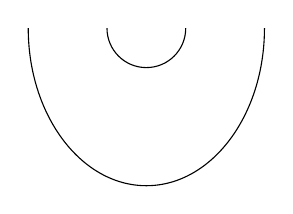
\begin{tikzpicture}

% open curve
\disk[](0,0)(2)(2);
\openGhost[](2,0)(1.5)(2)(2)();
\addGenus[](3,1)(40)(0.25);
\addGenus[](4.25,0.75)(-20)(0.25);

% doubled curve
\begin{scope}[xshift=8cm]
    \sphere[](0,0)(2)(2);
    \openGhost[](2,0)(1.5)(2)(2)();
    \draw (5,0) arc (0:-180:1.5 and 2);
    \draw (4,0) arc (0:-180:0.5 and 0.5);
    \addGenus[](3,1)(40)(0.25);
    \addGenus[](3,-1)(140)(0.25);
    \addGenus[](4.25,0.75)(-20)(0.25);
    \addGenus[](4.25,-0.75)(200)(0.25);
\end{scope}

\end{tikzpicture}
\caption{A curve modeled on $((2,2))$ and its genus $5$ double.}
\end{figure}
\end{remark}
